\chapter{Signals}

\epigraph{That's a signal, Jerry, that's a signal! [snaps his fingers again] Signal!}{George Costanza (Seinfeld)}

Signals are a convenient way to deliver low-priority information and for users to interact with their programs when other ways don't work (for example standard input being frozen).
They allow a program to clean up or perform an action in the case of an event.
Sometimes, a program can choose to ignore events which is supported.
Crafting a program that uses signals well is tricky due to how signals are handled.
As such, signals are usually for termination and clean up.
Rarely are they supposed to be used in programming logic.

For those of you with an architecture background, the interrupts used here aren't the interrupts generated by the hardware.
Those interrupts are almost always handled by the kernel because they require higher levels of privileges.
Instead, we are talking about software interrupts that are generated by the kernel -- though they can be in response to a hardware event like SIGSEGV.

This chapter will go over how to read information from a process that has either exited or been signaled.
Then, it will deep dive into what are signals, how does the kernel deal with a signal, and the various ways processes can handle signals both with and without threads.

\section{The Deep Dive of Signals}

A signal allows one process to asynchronously send an event or message to another process.
If that process wants to accept the signal, it can, and then, for most signals, decide what to do with that signal.

First, a bit of terminology.
A signal disposition is a per-process attribute that determines how a signal is handled after it is \textbf{delivered}.
Think of it as a table of signal-action pairs.
The full discussion is in the \href{http://man7.org/linux/man-pages/man7/signal.7.html}{Man Page}.
The actions are
\begin{enumerate}
  \item \keyword{TERM}, terminates the process
  \item \keyword{IGN}, ignore
  \item \keyword{CORE}, generate a core dump
  \item \keyword{STOP}, stops a process
  \item \keyword{CONT}, continues a process
  \item Execute a custom function.
\end{enumerate}

A signal mask determines whether a particular signal is delivered or not.
The overall process for how a kernel sends a signal are below.

\begin{enumerate}
\item If no signals have arrived, the process can install its own signal handlers.
  This tells the kernel that when the process gets signal X that it should jump to function Y.
\item A signal that is created is in a "generated" state.
\item The time between when a signal is generated and the kernel can apply the mask rules is called the pending state.
\item Then the kernel then checks the process' signal mask.
  If the mask says all the threads in a process are blocking the signal, then the signal is currently blocked and nothing happens until a thread unblocks it.
\item If a single thread can accept the signal, then the kernel executes the action in the disposition table.
  If the action is a default action, then no threads need to be paused.
\item Otherwise, the kernel delivers the signal by stopping \textit{whatever} a particular thread is doing currently, and jumps that thread to the signal handler.
  The signal is now in the delivered phase.
  More signals can be generated now, but they can't be delivered until the signal handler is complete which is when the delivered phase is over.
\item Finally, we consider a signal caught if the process remains intact after the signal was delivered.
\end{enumerate}

As a flowchart

\begin{figure}[H]
\centering
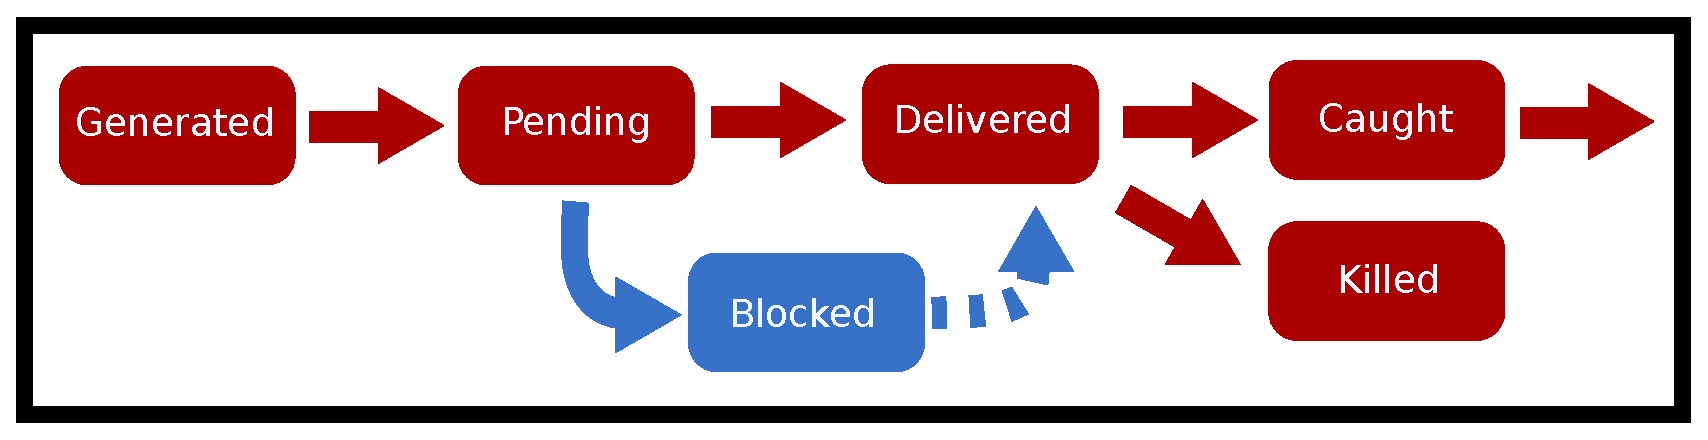
\includegraphics[width=.8\textwidth]{signals/drawings/signal_lifecycle.eps}
\caption{Signal lifecycle diagram}
\end{figure}

Here are some common signals that you will see thrown around.

\\
\begin{center}
\begin{table}[h]
\caption{POSIX Signals}
\begin{tabular}{|c|c|c|}
Name & Portable Number & Default Action & Usual Use \\ \hline
SIGINT & 2 & Terminate (Can be caught) & Stop a process nicely \\
SIGQUIT & 3 & Terminate (Can be caught) & Stop a process harshly \\
SIGTERM & 15 & Terminate Process & Stop a process even more harshly \\
SIGSTOP & N/A & Stop Process (Cannot be caught) & Suspends a process \\
SIGCONT & N/A & Continues a process & Starts after a stop \\
SIGKILL & 9 & Terminate Process (Cannot be caught) & You want the process gone
\end{tabular}
\end{table}
\end{center}
\\

One of our favorite anecdotes is to never use \keyword{kill -9} for a host of reasons.
The following is an excerpt from \underline{Useless Use of Kill -9} \href{http://porkmail.org/era/unix/award.html}{Link to archive}

\begin{quote}
No no no.  Don't use kill -9.

It doesn't give the process a chance to cleanly:

1) shut down socket connections

2) clean up temp files

3) inform its children that it is going away

4) reset its terminal characteristics

and so on and so on and so on.

Generally, send 15, and wait a second or two, and if that doesn't
work, send 2, and if that doesn't work, send 1.  If that doesn't,
REMOVE THE BINARY because the program is badly behaved!

Don't use kill -9.  Don't bring out the combine harvester just to tidy
up the flower pot.
\end{quote}

We still keep \keyword{kill -9} in there for extreme scenarios where the process needs to be gone.

\section{Sending Signals}

Signals can be generated in multiple ways.
\begin{enumerate}
\item The user can send a signal.
  For example, you are at the terminal, and you press \keyword{CTRL-C}.
  One can also use the built-in \keyword{kill} to send any signal.
\item The system can send an event.
For example, if a process accesses a page that it isn't supposed to, the hardware generates an interrupt which gets intercepted by the kernel.
The kernel finds the process that caused this and sends a software interrupt signal \keyword{SIGSEGV}.
There are other kernel events like a child being created or a process needs to be resumed.

\item Finally, another process can send a message.
  This could be used in low-stakes communication of events between processes.
  If you are relying on signals to be the driver in your program, you should rethink your application design.
  There are many drawbacks to using POSIX/Real-Time signals for asynchronous communication.
  The best way to handle interprocess communication is to use, well, interprocess communication methods specifically designed for your task at hand.
\end{enumerate}

You or another process can temporarily pause a running process by sending it a \keyword{SIGSTOP} signal.
If it succeeds, it will freeze a process.
The process will not be allocated any more CPU time.
To allow a process to resume execution, send it the SIGCONT signal.
For example, the following is a program that slowly prints a dot every second, up to 59 dots.

\begin{lstlisting}[language=C]
#include <unistd.h>
#include <stdio.h>
int main() {
  printf("My pid is %d\n", getpid() );
  int i = 60;
  while(--i) {
    write(1, ".",1);
    sleep(1);
  }
  write(1, "Done!",5);
  return 0;
}
\end{lstlisting}

We will first start the process in the background (notice the \& at the end).
Then, send it a signal from the shell process by using the kill command.

\begin{lstlisting}[language=bash]
$ ./program &
My pid is 403
...
$ kill -SIGSTOP 403
$ kill -SIGCONT 403
...
\end{lstlisting}

In C, a program can send a signal to the child using \keyword{kill} POSIX call,

\begin{lstlisting}[language=C]
kill(child, SIGUSR1); // Send a user-defined signal
kill(child, SIGSTOP); // Stop the child process (the child cannot prevent this)
kill(child, SIGTERM); // Terminate the child process (the child can prevent this)
kill(child, SIGINT); // The equivalent to CTRL-C (by default closes the process)
\end{lstlisting}

As we saw above there is also a \keyword{kill} command available in the shell.
Another command \keyword{killall} works the exact same way but instead of looking up by PID, it tries to match the name of the process.
\keyword{ps} is an important utility that can help you find the pid of a process.

\begin{lstlisting}[language=bash]
# First let's use ps and grep to find the process we want to send a signal to
$ ps au | grep myprogram
angrave  4409   0.0  0.0  2434892    512 s004  R+    2:42PM   0:00.00 myprogram 1 2 3

#Send SIGINT signal to process 4409 (The equivalent of `CTRL-C`)
$ kill -SIGINT 4409

# Send SIGKILL (terminate the process)
$ kill -SIGKILL 4409
$ kill -9 4409
# Use kill all instead to kill a process by executable name
$ killall -l firefox
\end{lstlisting}

To send a signal to the running process, use \keyword{raise} or \keyword{kill} with \keyword{getpid()}.

\begin{lstlisting}[language=C]
raise(int sig); // Send a signal to myself!
kill(getpid(), int sig); // Same as above
\end{lstlisting}

For non-root processes, signals can only be sent to processes of the same user.
You can't SIGKILL any process!
\keyword{man -s2 kill} for more details.

\section{Handling Signals}

There are strict limitations on the executable code inside a signal handler.
Most library and system calls are \keyword{async-signal-unsafe}, meaning they may not be used inside a signal handler because they are not re-entrant.
Re-entrant safety means that your function can be frozen at any point and executed again, can you guarantee that your function wouldn't fail?
Let's take the following

\begin{lstlisting}[language=C]
int func(const char *str) {
  static char buffer[200];
  strncpy(buffer, str, 199);
  # Here is where we get paused
  printf("%s\n", buffer)
}
\end{lstlisting}

\begin{enumerate}
\item We execute \keyword(func("Hello"))
\item The string gets copied over to the buffer completely (strcmp(buffer, "Hello") == 0)
\item A signal is delivered and the function state freezes, we also stop accepting any new signals until after the handler (we do this for convenience)
\item We execute \keyword{func("World")}
\item Now (strcmp(buffer, "World") == 0) and the buffer is printed out "World".
\item We resume the interrupted function and now print out the buffer once again "World" instead of what the function call originally intended "Hello"
\end{enumerate}

Guaranteeing that your functions are signal handler safe can't be solved by removing shared buffers.
You must also think about multithreading and synchronization -- what happens when I double lock a mutex?
You also have to make sure that each function call is reentrant safe.
Suppose your original program was interrupted while executing the library code of \keyword{malloc}.
The memory structures used by malloc will be inconsistent.
Calling \keyword{printf}, which uses \keyword{malloc} as part of the signal handler, is unsafe and will result in \textbf{undefined behavior}.
A safe way to avoid this behavior is to set a variable and let the program resume operating.
The design pattern also helps us in designing programs that can receive signals twice and operate correctly.

\begin{lstlisting}[language=C]
int pleaseStop ; // See notes on why "volatile sig_atomic_t" is better

void handle_sigint(int signal) {
  pleaseStop = 1;
}

int main() {
  signal(SIGINT, handle_sigint);
  pleaseStop = 0;
  while (!pleaseStop) {
    /* application logic here */
  }
  /* clean up code here */
}
\end{lstlisting}

The above code might appear to be correct on paper.
However, we need to provide a hint to the compiler and the CPU core that will execute the \keyword{main()} loop.
We need to prevent compiler optimization.
The expression \keyword{\!pleaseStop} doesn't get changed in the body of the loop, so some compilers will optimize it to \keyword{true} \todo{citation needed}.
Secondly, we need to ensure that the value of \keyword{pleaseStop} is uncached using a CPU register and instead always read from and written to main memory.
The \keyword{sig\_atomic\_t} type implies that all the bits of the variable can be read or modified as an \keyword{atomic operation} - a single uninterruptible operation.
It is impossible to read a value that is composed of some new bit values and old bit values.

By specifying \keyword{pleaseStop} with the correct type \keyword{volatile\ sig\_atomic\_t}, we can write portable code where the main loop will be exited after the signal handler returns.
The \keyword{sig\_atomic\_t} type can be as large as an \keyword{int} on most modern platforms but on embedded systems can be as small as a \keyword{char} and only able to represent (-127 to 127) values.

\begin{lstlisting}[language=C]
volatile sig_atomic_t pleaseStop;
\end{lstlisting}

Two examples of this pattern can be found in \keyword{COMP} a terminal based 1Hz 4bit computer \cite{Sorn_2015}.
Two boolean flags are used.
One to mark the delivery of \keyword{SIGINT} (CTRL-C), and gracefully shutdown the program, and the other to mark \keyword{SIGWINCH} signal to detect terminal resize and redraw the entire display.

You can also choose a handle pending signals asynchronously or synchronously.
To install a signal handler to asynchronously handle signals, use \keyword{sigaction}.
To synchronously catch a pending signal use \keyword{sigwait} which blocks until a signal is delivered or \keyword{signalfd} which also blocks and provides a file descriptor that can be \keyword{read()} to retrieve pending signals.

\subsection{Sigaction}

You should use \keyword{sigaction} instead of \keyword{signal} because it has better defined semantics.
\keyword{signal} on different operating system does different things which is \textbf{bad}.
\keyword{sigaction} is more portable and is better defined for threads.
You can use system call \keyword{sigaction} to set the current handler and disposition for a signal or read the current signal handler for a particular signal.

\begin{lstlisting}[language=C]
int sigaction(int signum, const struct sigaction *act, struct sigaction *oldact);
\end{lstlisting}

The sigaction struct includes two callback functions (we will only look at the `handler' version), a signal mask and a flags field -

\begin{lstlisting}[language=C]
struct sigaction {
  void     (*sa_handler)(int);
  void     (*sa_sigaction)(int, siginfo_t *, void *);
  sigset_t   sa_mask;
  int        sa_flags;
};
\end{lstlisting}

Suppose you stumble upon legacy code that uses \keyword{signal}.
The following snippet installs \keyword{myhandler} as the SIGALRM handler.

\begin{lstlisting}[language=C]
signal(SIGALRM, myhandler);
\end{lstlisting}

The equivalent \keyword{sigaction} code is:

\begin{lstlisting}[language=C]
struct sigaction sa;
sa.sa_handler = myhandler;
sigemptyset(&sa.sa_mask);
sa.sa_flags = 0;
sigaction(SIGALRM, &sa, NULL)
\end{lstlisting}

However, we typically may also set the mask and the flags field.
The mask is a temporary signal mask used during the signal handler execution.
If the thread serving the signal is interrupted in the middle of a system call, the \keyword{SA\_RESTART} flag will automatically restart some system calls that otherwise would have returned early with EINTR error.
The latter means we can simplify the rest of code somewhat because a restart loop may no longer be required.

\begin{lstlisting}[language=C]
sigfillset(&sa.sa_mask);
sa.sa_flags = SA_RESTART; /* Restart functions if interrupted by handler */
\end{lstlisting}

It is often better to have your code check for the error and restart itself due to the selective nature of the flag.

\section{Blocking Signals}

To block signals use \keyword{sigprocmask}!
With sigprocmask you can set the new mask, add new signals to be blocked to the process mask, and unblock currently blocked signals.
You can also determine the existing mask (and use it for later) by passing in a non-null value for oldset.

\begin{lstlisting}[language=C]
int sigprocmask(int how, const sigset_t *set, sigset_t *oldset);
\end{lstlisting}

From the Linux man page of sigprocmask, here are the possible values for \keyword{how} \todo{cite}.

\begin{itemize}
\item \keyword{SIG\_BLOCK}.
  The set of blocked signals is the union of the current set and the set argument.
\item \keyword{SIG\_UNBLOCK}.
  The signals in set are removed from the current set of blocked signals.
  It is permissible to attempt to unblock a signal which is not blocked.
\item \keyword{SIG\_SETMASK}.
  The set of blocked signals is set to the argument set.
\end{itemize}

The sigset type behaves as a set.
It is a common error to forget to initialize the signal set before adding to the set.

\begin{lstlisting}[language=C]
sigset_t set, oldset;
sigaddset(&set, SIGINT); // Ooops!
sigprocmask(SIG_SETMASK, &set, &oldset)
\end{lstlisting}

Correct code initializes the set to be all on or all off. For example,

\begin{lstlisting}[language=C]
sigfillset(&set); // all signals
sigprocmask(SIG_SETMASK, &set, NULL); // Block all the signals which can be blocked

sigemptyset(&set); // no signals
sigprocmask(SIG_SETMASK, &set, NULL); // set the mask to be empty again
\end{lstlisting}

If you block a signal with either \keyword{sigprocmask} or \keyword{pthread\_sigmask}, then the handler registered with \keyword{sigaction} is not delivered unless explicitly \keyword{sigwait'ed} on \todo{cite}.

\subsection{Sigwait}

Sigwait can be used to read one pending signal at a time.
\keyword{sigwait} is used to synchronously wait for signals, rather than handle them in a callback.
A typical use of sigwait in a multi-threaded program is shown below.
Notice that the thread signal mask is set first (and will be inherited by new threads).
The mask prevents signals from being \emph{delivered} so they will remain in a pending state until sigwait is called.
Also notice the same set \keyword{sigset\_t} variable is used by sigwait - except rather than setting the set of blocked signals it is used as the set of signals that sigwait can catch and return.

One advantage of writing a custom signal handling thread (such as the example below) rather than a callback function is that you can now use many more C library and system functions safely.

Based on sigmask code \cite{pthread_sigmask}

\begin{lstlisting}[language=C]
static sigset_t signal_mask; /* signals to block */

int main(int argc, char *argv[]) {
  pthread_t sig_thr_id; /* signal handler thread ID */
  sigemptyset (&signal_mask);
  sigaddset (&signal_mask, SIGINT);
  sigaddset (&signal_mask, SIGTERM);
  pthread_sigmask (SIG_BLOCK, &signal_mask, NULL);

  /* New threads will inherit this thread's mask */
  pthread_create (&sig_thr_id, NULL, signal_thread, NULL);

  /* APPLICATION CODE */
  ...
}

void *signal_thread(void *arg) {
  int sig_caught;

  /* Use the same mask as the set of signals that we'd like to know about! */
  sigwait(&signal_mask, &sig_caught);
  switch (sig_caught) {
    case SIGINT:
    ...
    break;
    case SIGTERM:
    ...
    break;
    default:
    fprintf (stderr, "\nUnexpected signal %d\n", sig_caught);
    break;
  }
}
\end{lstlisting}

\section{Signals in Child Processes and Threads}

This is a recap of the processes chapter.
After forking, the child process inherits a copy of the parent's signal dispositions and a copy of the parent's signal mask.
If you have installed a SIGINT handler before forking, then the child process will also call the handler if a SIGINT is delivered to the child.
If \keyword{SIGINT} is blocked in the parent, it will be blocked in the child as well.
Note that pending signals for the child are \emph{not} inherited during forking.
After \keyword{exec} though, only the signal mask and pending signals are carried over \cite{execute}.
Signal handlers are reset to their original action, because the original handler code may have disappeared along with the old process.

Each thread has its own mask.
A new thread inherits a copy of the calling thread's mask.
On initialization, the calling thread's mask is the exact same as the processes mask.
After a new thread is created though, the processes signal mask turns into a gray area.
Instead, the kernel likes to treat the process as a collection of threads, each of which can institute a signal mask and receive signals.
To start setting your mask, you can use,

\begin{lstlisting}[language=C]
pthread_sigmask(...); // set my mask to block delivery of some signals
pthread_create(...); // new thread will start with a copy of the same mask
\end{lstlisting}

Blocking signals is similar in multi-threaded programs to single-threaded programs with the following translation.

\begin{enumerate}
\item Use \keyword{pthread\_sigmask} instead of \keyword{sigprocmask}
\item Block a signal in all threads to prevent its asynchronous delivery
\end{enumerate}

The easiest method to ensure a signal is blocked in all threads is to set the signal mask in the main thread before new threads are created.

\begin{lstlisting}[language=C]
sigemptyset(&set);
sigaddset(&set, SIGQUIT);
sigaddset(&set, SIGINT);
pthread_sigmask(SIG_BLOCK, &set, NULL);

// this thread and the new thread will block SIGQUIT and SIGINT
pthread_create(&thread_id, NULL, myfunc, funcparam);
\end{lstlisting}

Just as we saw with \keyword{sigprocmask}, \keyword{pthread\_sigmask} includes a `how' parameter that defines how the signal set is to be used:

\begin{lstlisting}[language=C]
pthread_sigmask(SIG_SETMASK, &set, NULL) - replace the thread's mask with given signal set
pthread_sigmask(SIG_BLOCK, &set, NULL) - add the signal set to the thread's mask
pthread_sigmask(SIG_UNBLOCK, &set, NULL) - remove the signal set from the thread's mask
\end{lstlisting}

A signal then can be delivered to any signal thread that is willing to accept that signal.
If the two or more threads can receive the signal then which thread will be interrupted is arbitrary!
A common practice is to have one thread that can receive all signals or if there is a certain signal that requires special logic, have multiple threads for multiple signals.
Even though programs from the outside can't send signals to specific threads, you can do that internally with \keyword{pthread\_kill(pthread\_t thread, int sig)}.
In the example below, the newly created thread executing \keyword{func} will be interrupted by \keyword{SIGINT}

\begin{lstlisting}[language=C]
pthread_create(&tid, NULL, func, args);
pthread_kill(tid, SIGINT);
pthread_kill(pthread_self(), SIGKILL); // send SIGKILL to myself
\end{lstlisting}

As a word of warning \keyword{pthread\_kill(threadid, SIGKILL)} will kill the entire process.
Though individual threads can set a signal mask, the signal disposition is \emph{per-proces}s not \emph{per-thread}.
This means \keyword{sigaction} can be called from any thread because you will be setting a signal handler for all threads in the process.

The Linux man pages discuss signal system calls in section 2. There is also a longer article in section 7 (though not in OSX/BSD):

\begin{lstlisting}[language=C]
man -s7 signal
\end{lstlisting}

\section{Topics}

\begin{itemize}
\tightlist
\item
  Signals
\item
  Signal Handler Safety
\item
  Signal Disposition
\item
  Signal States
\item
  Pending Signals when Forking/Exec
\item
  Signal Disposition when Forking/Exec
\item
  Raising Signals in C
\item
  Raising Signals in a multithreaded program
\end{itemize}

\section{Questions}

\begin{itemize}
\tightlist
\item
  What is a signal?
\item
  How are signals served under UNIX? (Bonus: How about Windows?)
\item
  What does it mean that a function is signal handler safe? How about reentrant?
\item
  What is a process signal disposition? How does it differ from a mask?
\item
  What function changes the signal disposition in a single threaded program?
  How about a multithreaded program?
\item
  What are some drawbacks to using signals?
\item
  What are the ways of asynchronously and synchronously catching a signal?
\item
  What happens to pending signals after a fork? exec? How about my signal mask? How about signal disposition?
\item
  What is the process the kernel goes through from creation to delivery/block?
\end{itemize}

\bibliographystyle{plainnat}
\bibliography{signals/signals}
